\documentclass[11pt,titlepage]{article}
\usepackage[utf8]{inputenc}
\usepackage[margin=1.0in]{geometry}
\usepackage{graphicx}
\usepackage{subfigure}
\usepackage{amssymb,amsfonts,amsmath}
\usepackage{url}
\usepackage{booktabs, multicol, multirow}
\usepackage[round,numbers,sort&compress]{natbib}

% Bibliography style (requires the style file biophysj.bst in the 
% document directory)
\bibliographystyle{biophysj}

\author{Kyle A. Beauchamp, \\
Biophysics Program, \\
Stanford University, Stanford, CA
\and Rhiju Das \\
Biochemistry and Physics Departments, \\
Stanford University, Stanford, CA
\and Vijay S. Pande, \\
Chemistry Department and Structural Biology Program, \\
Stanford University, Stanford, CA
}


\title{Removing Force Field Bias from Structural Ensembles Inferred from Noisy Experiments and Molecular Dynamics}

\begin{document}

\maketitle

\begin{abstract}

Inferring biomolecular conformation from experiment is the fundamental goal of structural biology.  Structure determination often requires the combination of modeling and experiment, but the vast majority of approaches model only a single conformation, provide limited uncertainty information, and inherit biases from assumed force fields when data are limited.  Building on conceptual advances by Pitera and Chodera, we describe and test Bayesian Energy Landscape Tilting (BELT), a scheme that  leverages Bayesian statistics to model conformational ensembles with uncertainty estimates derived from an independent normal error model.  BELT corrects force field bias in a trialanine test system, as assessed by the convergence of $\alpha$, $\beta$, and $PP_{II}$ conformational populations in ensembles constructed by combining scalar coupling and chemical shift measurements with simulations performed in five different force fields (ff96, ff99, ff99sbnmr-ildn, charmm27, and oplsasa).  As a test of predictive power, BELT modeling with a subset of six NMR measurements recovers, within prediction error, three datapoints not used during fitting.  The principled combination of simulation and limited experimental data promises equilibrium and structural models not previously possible with simulation or experiment alone.  

\end{abstract}

\emph{Key words:} Molecular Dynamics, NMR, Conformational Ensembles,  Bayesian Statistics

\section*{Introduction}

Over the past forty years, structural biologists have solved ``ground-state'' structures of countless biological macromolecules \citep{Berman2000}. Modern biology, however, presents many systems that do not fit the single-structure paradigm.  Excited states of nucleic acids \citep{dethoff2012}, natively disordered proteins \citep{fink2005}, and protein folding intermediates \citep{korzhnev2004} alike are poorly described by single conformation models.  For such systems, models of conformational ensembles are required to understand and predict structural and equilibrium properties.  

A growing body of research has sought to characterize structural ensembles.  Much of it has focused on incorporating dynamical information during NMR structure determination  \citep{lindorff2005simultaneous, lange2008recognition} or the extraction of multiple conformers from X-ray diffraction data  \citep{depristo2004heterogeneity, lang2010automated}.  While these techniques are powerful, they share difficulties in data collection and the unified treatment of heterogeneous experimental data.  

Conformational ensemble modeling requires the estimation of not just a single structure, but a collection of structures and their associated equilibrium populations.  This highly under-determined problem involves the simultaneous estimation of approximately $m\times 3N$ parameters, $m$ is the number of states in the ensemble and $N$ is the number of atoms in the model.  Inference in this regime necessarily requires some additional information, which is provided by combining measurements with information provided by an atomistic force field.  However, simulation studies have demonstrated possible inaccuracies in molecular dynamics force fields \citep{best2008, lindorff2012systematic, beauchamp2012protein}.  Force field modifications based on direct fitting to NMR measurements have also been demonstrated \cite{li2011iterative, best2012optimization, nerenberg2011}, but such work has typically fit to only a handful of measurements that are most sensitive to torsional force field terms.  Often, however, one desires to have atomic-scale models that are both consistent with presently available measurements and predictive of those yet to be measured.  

Here we introduce a statistical approach to modeling solution ensembles of biological macromolecules.  The algorithm, Bayesian Energy Landscape Tilting (BELT), uses solution experiments to reweight a collection of atomistic models.  BELT extends a recent maximum entropy method for restraining simulations  \citep{chodera2012} to reweight existing simulations.  Furthermore, BELT leverages Markov Chain Monte Carlo to transform experimental ambiguity into error bars on arbitrary structural features.  

One stringent validation of BELT is to assess the convergence of ensembles constructed from force fields with radically different properties.  We therefore investigated the conformational propensities of trialanine using NMR measurements \citep{Graf2007} and MD simulations performed in five different force fields.  Although the raw simulations show wide variations in their conformational preferences, BELT corrects force field errors to provide self-consistent estimates of the $\alpha$, $\beta$, and $PP_{II}$ populations.  The ability to correct the biases of all tested forcefields suggests that BELT is a powerful technique for connecting simulation and equilibrium measurements.  

\section*{Theory: Bayesian Energy Landscape Tilting}

\subsection*{Model Inputs}

To model an ensemble using BELT requires three components (Fig. \ref{figure:BELT}).  First, we need conformations $(x_j)_{j=1}^{m}$ sampled from the equilibrium distribution of some physically realistic model.  This model will serve as a prior on structural properties; in the absence of experimental data, the BELT model inherits the properties of the prior simulations $x_j$.  In the present work, such conformations will be generated from molecular dynamics simulations.  Second, we require equilibrium experimental measurements $(F_i)_{i=1}^n$ and their associated uncertainties $(\sigma_i)_{i=1}^{n}$.  Third, it is necessary to have a direct connection between simulation and experiment.  This connection is achieved by predicting each experimental observable at each conformation: $f_i(x_j)$ is the predicted value of experiment $i$ at conformation $x_j$.  

\begin{figure}

\includegraphics[width=16.0cm]{figures/info_graphic/info_graphic.png}

\caption{
General scheme for BELT modeling.
}
\label{figure:BELT}
\end{figure}

\subsection*{Reweighting}

The next step in constructing an ensemble is to calculate the population of each conformation.  For convenience, we work with the $\log$ populations (i.e. free energies scaled such that the thermal energy $k_B T$ is unity). Inspired by a previous method for restraining simulations  \citep{chodera2012} (see Appx. S1), we reweight individual conformations by a biasing potential that is a linear combination of the predicted observables:

$$\Delta U(x;\alpha) = \sum_{i=1}^n \alpha_i f_i(x)$$

In $\Delta U(x;\alpha)$, the parameters $\alpha_i$ determine how strongly each experiment contributes to the biasing potential.  One way to think about each $\alpha_i$ is via ``tilting'' the energy landscape along the order parameters $f_i(x)$.  Given the biasing potential, the population of each conformation can be calculated using exponential averaging (see Appx. S2):

$$\pi_j(\alpha) = \frac{1}{\sum_k \exp[-\Delta U(x_k;\alpha)]} \exp[-\Delta U(x_j;\alpha)]$$

It is informative to consider the case of a single observable $f_1(x)$ (and therefore a single parameter $\alpha_1$).  Suppose the molecule of interest shows a bimodal observable with two equally populated states.  If we let $\alpha_1$ = 0, then the biasing potential is $0$ everywhere and our reweighted ensemble simply returns the results of the MD simulation (Fig. \ref{figure:Hist}b).  If we let $\alpha_1 = -1$, conformations with large values of $f_1(x)$ are upweighted, while conformations with lower values of $f_1(x)$ are downweighted (Fig. \ref{figure:Hist}a).  Finally, if $\alpha_1 = 1$, the ensemble shifts in the opposite direction (Fig. \ref{figure:Hist}c).  

\begin{figure}

\subfigure[]{
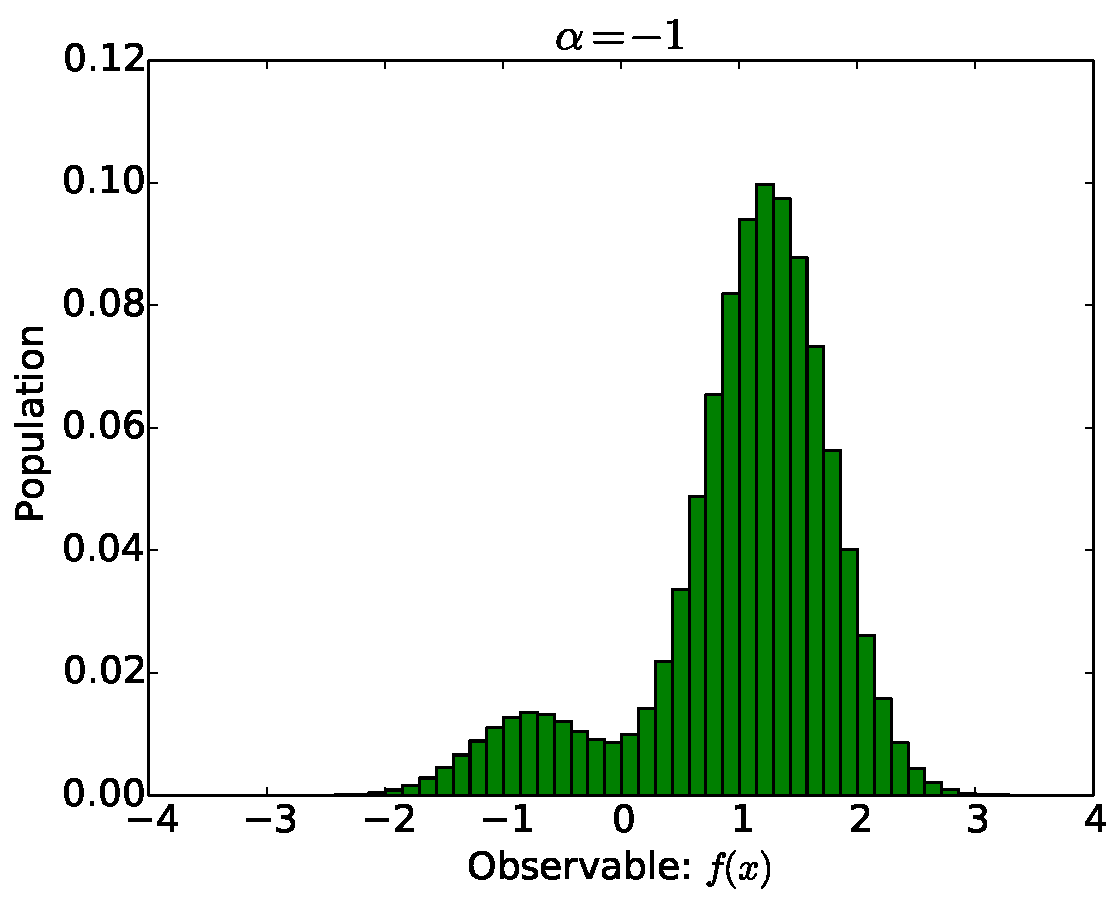
\includegraphics[width=5.0cm]{figures/model_hist-1.pdf}
}
\subfigure[]{
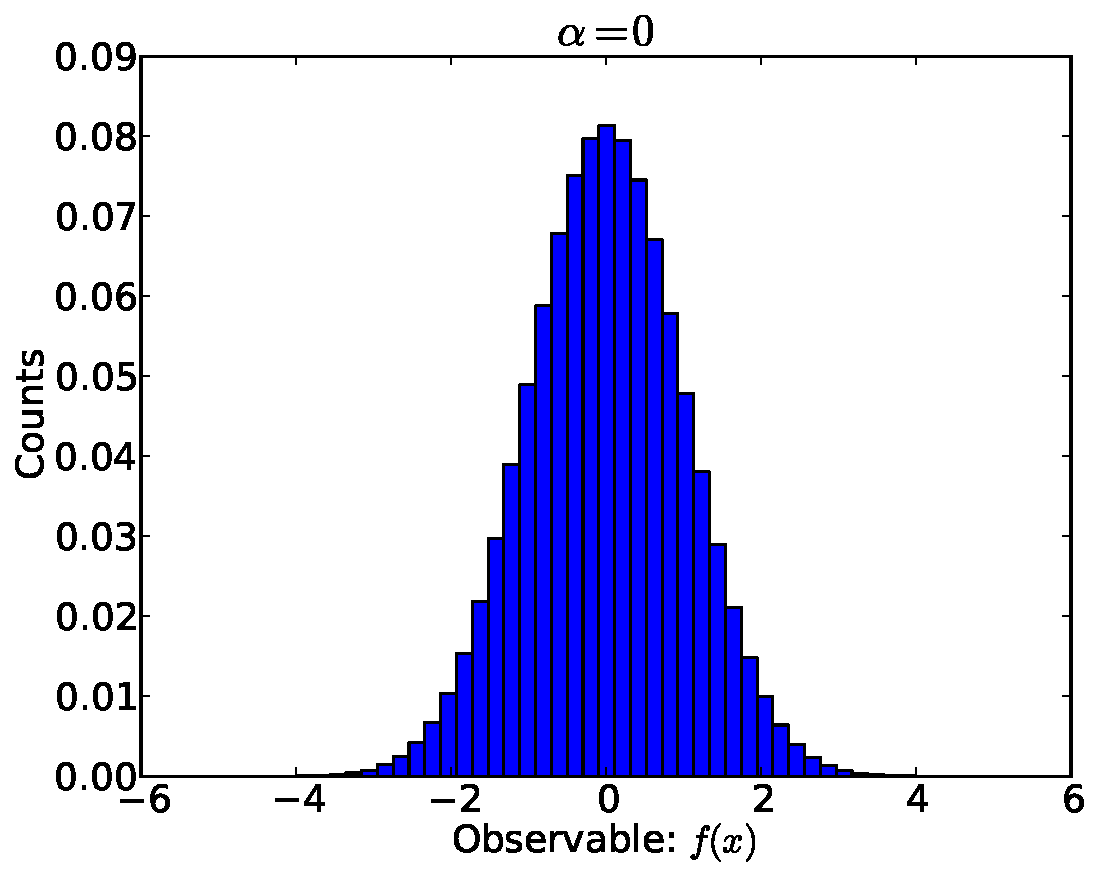
\includegraphics[width=5.0cm]{figures/model_hist0.pdf}
}
\subfigure[]{
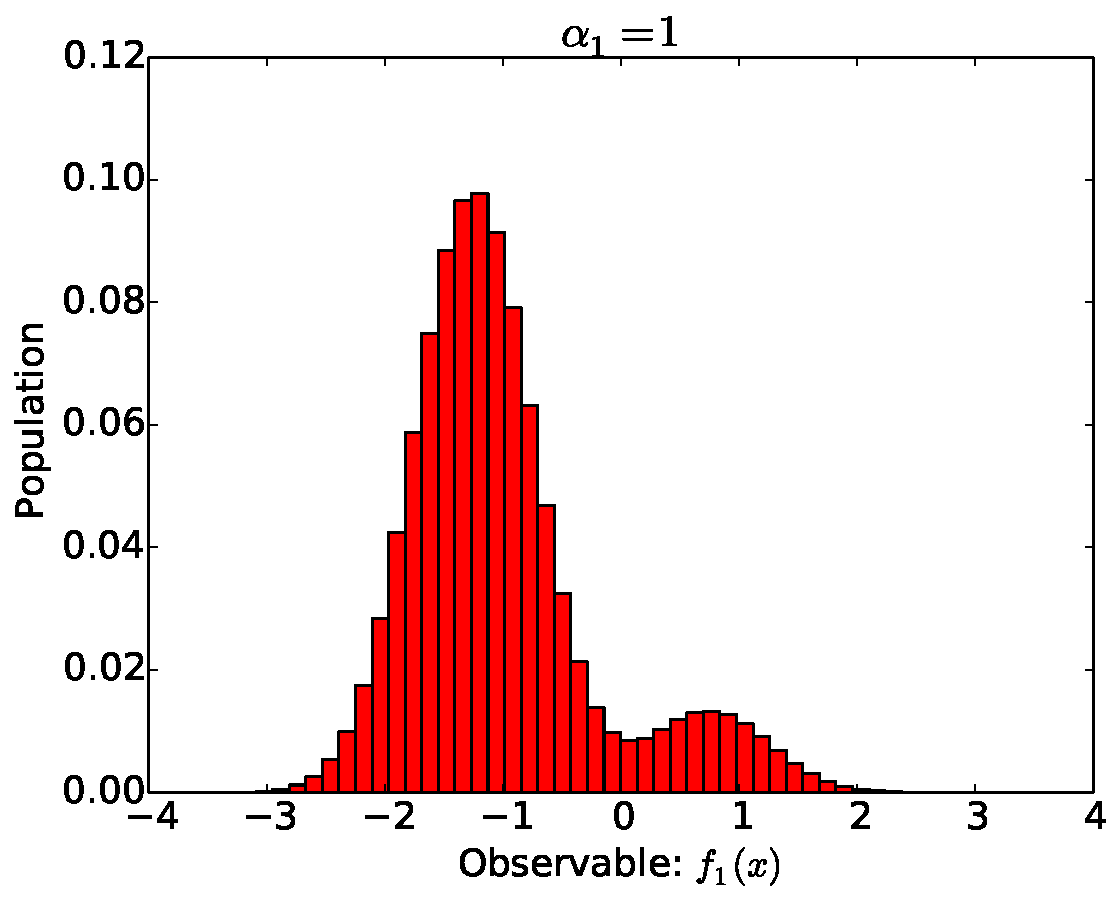
\includegraphics[width=5.0cm]{figures/model_hist1.pdf}
}
\caption{
Raw ($\alpha_1 = 0$) and reweighted (e.g. tilted) histograms of a one dimensional observable.
}
\label{figure:Hist}
\end{figure}

With the equilibrium populations, we can calculate the equilibrium expectations of an arbitrary observable $h(x)$:

$$\langle h(x)\rangle _\alpha = \sum_j h(x_j) \pi_j(\alpha)$$

In the above bracket notation, $\langle h(x)\rangle _\alpha$ is the ensemble average of $h(x)$ in an ensemble that is perturbed by a biasing potential $\Delta U(x;\alpha)$.  At this point, the determination of the parameters $\alpha_i$ has not yet been discussed.  The key idea, however, is that the $\alpha$ reweighted ensemble $\langle \rangle _\alpha$ should recapitulate the experimental measurements:

$$\langle f_i(x)\rangle _\alpha \approx F_i$$

Forcing this to be an exact equality recovers previous results \citep{chodera2012} that can be derived from maximum entropy considerations (Appx. S1); here, however, we take into account the experimental uncertainties associated with each $F_i$.  

\subsection*{Determining $\alpha$}

We now derive a Bayesian framework for determining the coefficients $\alpha$ used in the biasing potential.  Given adequate sampling and self-consistent experiments, there should exist some true value of $\alpha$ whose ensemble matches the experimental data.  However, experimental uncertainty ($\sigma_i)$ prevents exact agreement between the measurements and the true ensemble.  For the models in the current work, we model $\sigma_i$ as the uncertainty associated with predicting chemical shifts and scalar couplings from structures; this dominant error is quantified by the RMS uncertainty estimated during the parameterization of chemical shift and scalar coupling models.  We use an independent normal approximation (see Appx. S3) to model the likelihood of the model specified by $\alpha$:

$$P(F_i | \alpha) \sim N(\langle f_i(x)\rangle _\alpha, \sigma_i^2)$$

Using Bayes' Theorem, we can calculate the posterior distribution of $\alpha$:

$$P(\alpha | F_1, ..., F_n) \propto P(F_1, ..., F_n | \alpha) P(\alpha)$$

Now we let $LP(\alpha)$ denote the log posterior of $\alpha$ and simplify, dropping terms that are independent of $\alpha$:

$$LP(\alpha) = \log[ P(\alpha|F_1, ..., F_n)] = -\sum_i^n \frac{1}{2\sigma_i^2}(\langle f_i(x)\rangle _\alpha - F_i)^2 + \log P(\alpha) + constant$$

Note the simple form of the log posterior.  The first term (i.e. the log likelihood) measures the $\chi^2$ agreement between the reweighted ensemble and measurements.  The second term is the log of the prior distribution on $\alpha$.  

In the present work, we evaluate three different choices of prior (Appx. S4), finding similar results for each.  The first is the maximum entropy (maxent) prior, which penalizes ensembles as they deviate from the raw simulation results:

$$\log P(\alpha) = -\lambda \sum_j^m \pi_j(\alpha) \log \frac{\pi_j(\alpha)}{\pi_j^0}$$

In the previous expression, $\pi_j^0$ refers to the populations of an unweighted ensemble, which are typically $\frac{1}{m}$.  We also consider using a Dirichlet prior, which is functionally similar to the maxent (Appx. S4):

$$\log P(\alpha) = -\lambda \sum_j \pi_j^0 \log \frac{\pi_j^0}{\pi_j(\alpha)}$$

The third prior we consider is a multivariate normal prior, where  $\alpha \sim N(0, \Sigma)$.  The value of $\Sigma$ is given by $\Sigma_{ij} = \lambda Cov(f_i(x), f_j(x))$, as derived in Appx. S4.

These priors can be used to achieve regularization, which is a powerful technique to reduce overfitting \cite{friedman2001elements}.  Large values of $\lambda$ favor the raw simulation results (i.e. uniform conformational populations): $\pi_j \approx \pi_j^0 = \frac{1}{m}$.  The value of $\lambda$ can be chosen via cross-validation or other methods (see Appx. S5).  

\subsection*{MCMC Sampling of Structural Ensembles}

Because ensemble inference often presents many plausible solutions  \citep{fisher2010, rieping2005}, we avoid statistical methods that return a single solution (e.g. maximum likelihood).  We therefore use Markov chain Monte Carlo (MCMC), as implemented in PyMC  \citep{patil2010pymc}, to sample the distribution of structural ensembles consistent with experiment.  The result is an ensemble of ensembles--a statistical ensemble of conformational ensembles.  Averaging all MCMC samples provides posterior mean  estimates of arbitrary structural features.  Similarly, examining the MCMC variances provides statistical uncertainties of equilibrium or structural features.  A Bayesian bootstrapping procedure  \citep{rubin1981} can also be used to model the statistical uncertainty of the MD simulations (see Appx. S6).

\section*{Methods}

\subsection*{Molecular Dynamics Simulations}

Trialanine was simulated in the amber96 \citep{kollman1996}, amber99 \citep{wang2000}, amber99sbnmr-ildn \citep{li2010, Lindorff-Larsen2010}, charmm27 \citep{mackerell2004extending,bjelkmar2010implementation}, and oplsaa \citep{kaminski2001evaluation} force fields, as previously reported  \citep{beauchamp2012protein}.  Simulations were performed using Gromacs 4.5  \citep{hess2008} and run at constant temperature (300 K) and pressure (1.01 atm).  Each simulation was at least 225 ns long.  Conformations were stored every 1 ps.  

\subsection*{Chemical Shifts and Scalar Couplings}

All NMR measurements in this work refer to experiments  \citep{Graf2007} probing the central residue of trialanine.  Because the experimental data was measured at pH 2, which lies near the pKa of the C terminus.  This indicates that the true ensemble likely requires a constant pH simulation, rather than a fixed protonation state.  However, such simulations are challenging with current force fields and simulation packages, so we therefore focus our analysis on the central alanine residue.  

Chemical shifts ($H$, $H_\alpha$, $C_\alpha$, $C_\beta$) for each frame were calculated using a weighted average of ShiftX2 \citep{han2011shiftx2}, SPARTA+  \citep{Shen2010}, and PPM \citep{li2012ppm} predictions; uncertainties for each model were estimated using their reported RMS prediction errors.  Overall uncertainties were estimated as $\sqrt{\sum w_i \sigma_i^2}$, where $w_i \propto \frac{1}{\sigma_i^2}$ is the weight (e.g $\sum_i w_i = 1$) of each chemical shift model and $\sigma_i$ is the uncertainty of each chemical shift model.  The J couplings were calculated using the following Karplus relations: $^3J(H^N C')$  \citep{vogeli2007limits}, $^3J(H^N H^\alpha)$  \citep{vogeli2007limits}, $^2J(N C^\alpha)$  \citep{Graf2007}, $^3J(H^\alpha C')$  \citep{Schmidt1999}, $^1J(N C^\alpha)$  \citep{Graf2007}, $^3J(H^N C^\beta)$  \citep{vogeli2007limits}.  J coupling uncertainties were approximated as the RMS errors reported when fitting the Karplus coefficients.  

We have divided the available experimental measurements into a training and test set, with the training set consisting of the $^3J(H^N C')$,  $^2J(N C^\alpha)$, and $^3J(H^N C^\beta)$ scalar couplings and the $C_\alpha$, $H$, and $C_\beta$ chemical shifts.  The test set consists of $^3J(H^N H^\alpha)$, $^3J(H^\alpha C')$, and $^1J(N C^\alpha)$.  The division into training and test sets serves three purposes.  First, it provides a test of overfitting.  Second, it allows us to reduce the computational cost of BELT calculations.  Third, it allows us to train on data that are approximately uncorrelated; BELT is best suited for working with uncorrelated data.  Additional suggestions for data curation are provided in Appx. S7.  

\subsection*{BELT}

All BELT calculations were performed using the FitEnsemble package (\url{https://github.com/kyleabeauchamp/FitEnsemble}).  The online FitEnsemble tutorial demonstrates the use of BELT with a single experimental measurement ($^3J(H^N H^\alpha)$).  Source code for calculations in this work will be made available at \url{https://github.com/kyleabeauchamp/EnsemblePaper}.  

Regularization strength was determined via cross validation as described in Appx. S5.  For each model, we used PyMC to sample at least 5,000,000 values of $\alpha$; sampled values of $\alpha$ were thinned 100-fold to reduce correlation.  The first 5,000 samples (before thinning) are discarded as burn-in.  MCMC traces are shown in Fig. S2 and discussed in Appx. S8.  To incorporate simulation uncertainty, we used Bayesian Bootstrapping (Appx. S6).  Two Bayesian bootstrap replicates were performed.  

\section*{Results}

\subsection*{Conformational Propensities of Trialanine}

Short peptides provide crucial tests for evaluating and optimizing molecular dynamics force fields  \citep{Graf2007,beauchamp2012protein, nerenberg2011, best2008, Grdadolnik2011}.  Such peptides offer a window into the intrinsic conformational propensities of amino acids, free from the secondary structure bias found in statistical surveys of protein structures  \citep{Jha2005}.  Here, we use BELT to infer the conformational populations of trialanine from chemical shift and scalar coupling measurements  \citep{Graf2007}.  

Trialanine was simulated (see Methods) in five different force fields; six experimental measurements (three scalar couplings, three chemical shifts) probing the central alanine residue were used to construct a BELT ensemble.  The five force fields show considerable variation in their agreement with experiment (Fig. \ref{figure:ChiSquared}).  The amber96, amber99, charmm27, and oplsaa force fields, for example, initially show significant deviation from the experimental measurements.  Upon reweighting, however, all five force fields agree with experiment--including experiments that were not used to fit the model (Fig. \ref{figure:ChiSquared}b).  Additionally, these results are robust to differences in the prior placed on $\alpha$.

\begin{figure}
\subfigure[]{
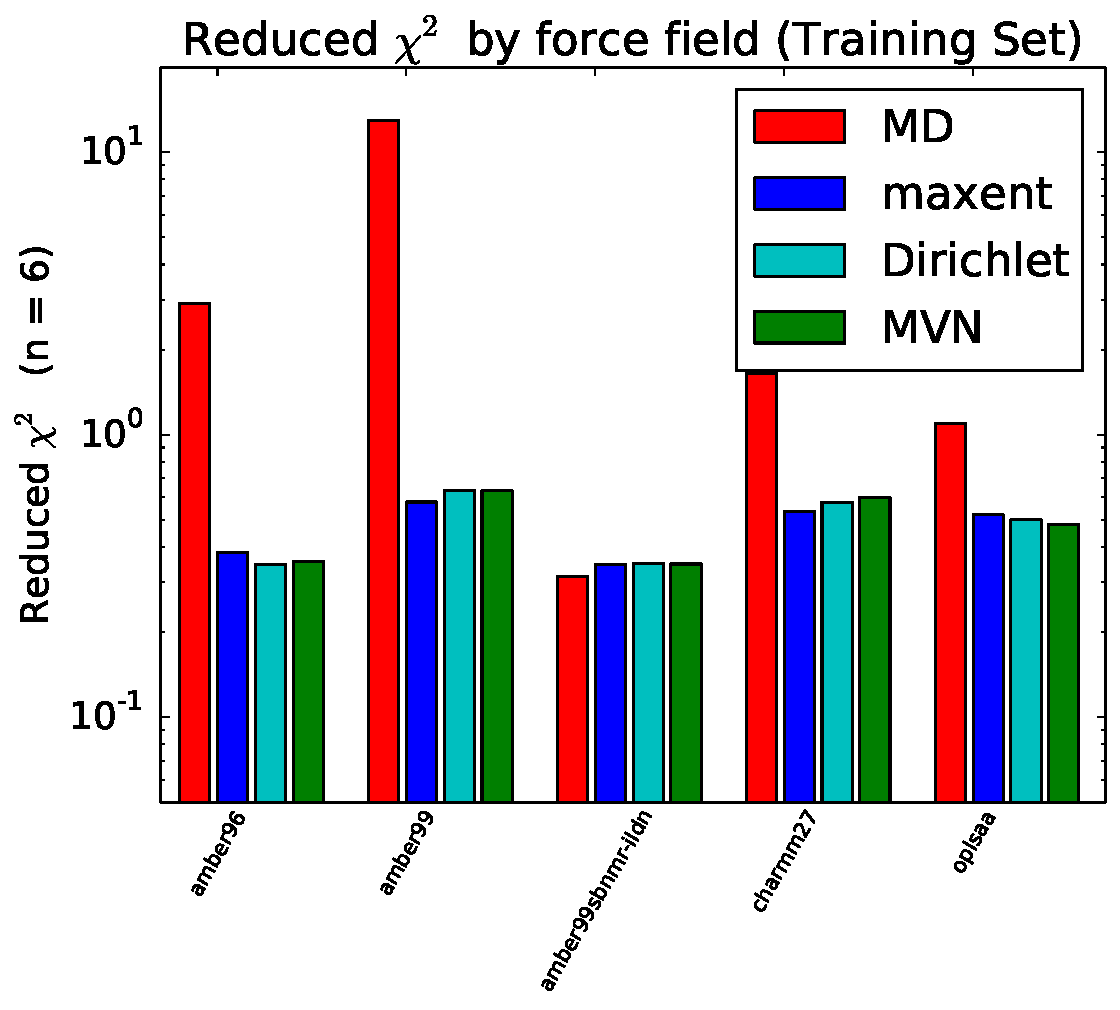
\includegraphics[width=7.5cm]{figures/chi2_train_priors.pdf}
}
\subfigure[]{
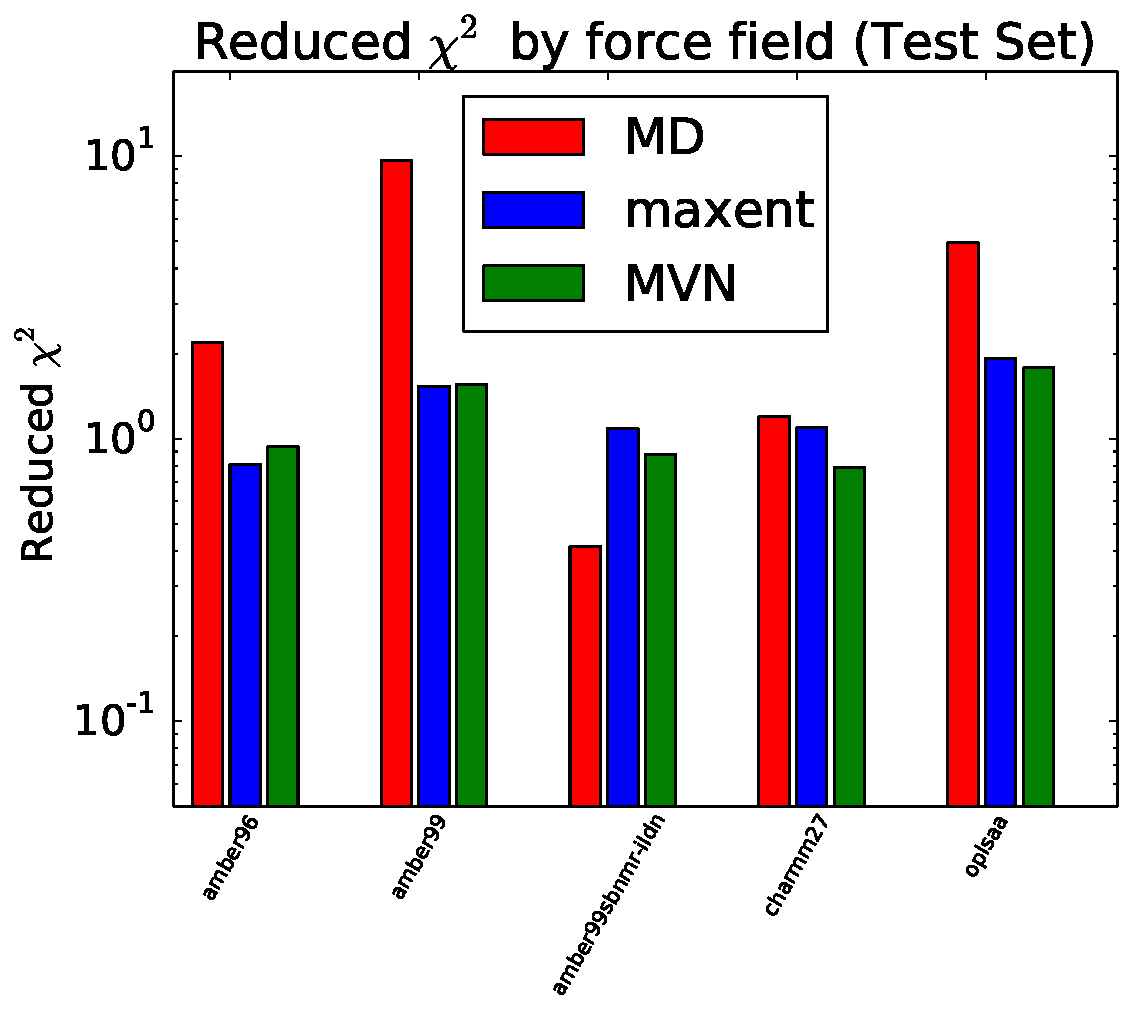
\includegraphics[width=7.5cm]{figures/chi2_test_priors.pdf}
}
\caption{
The reduced $\chi^2$ error (e.g. $\frac{\chi^2}{n}$) for MD and BELT (maxent, Dirichlet, and MVN priors) models.  The BELT reduced $\chi^2$ is estimated as the mean reduced $\chi^2$ over all MCMC samples.  (a).  Calculated using the six measurements used to fit the BELT model.  (b).  Calculated using four measurements not used to fit the BELT model.  See Methods for the definition of training and test sets.  Note that the training and test sets are not fully independent because all measurements probe the $(\phi, \psi)$ backbone torsions.
}
\label{figure:ChiSquared}
\end{figure}



\begin{figure}
\subfigure[]{
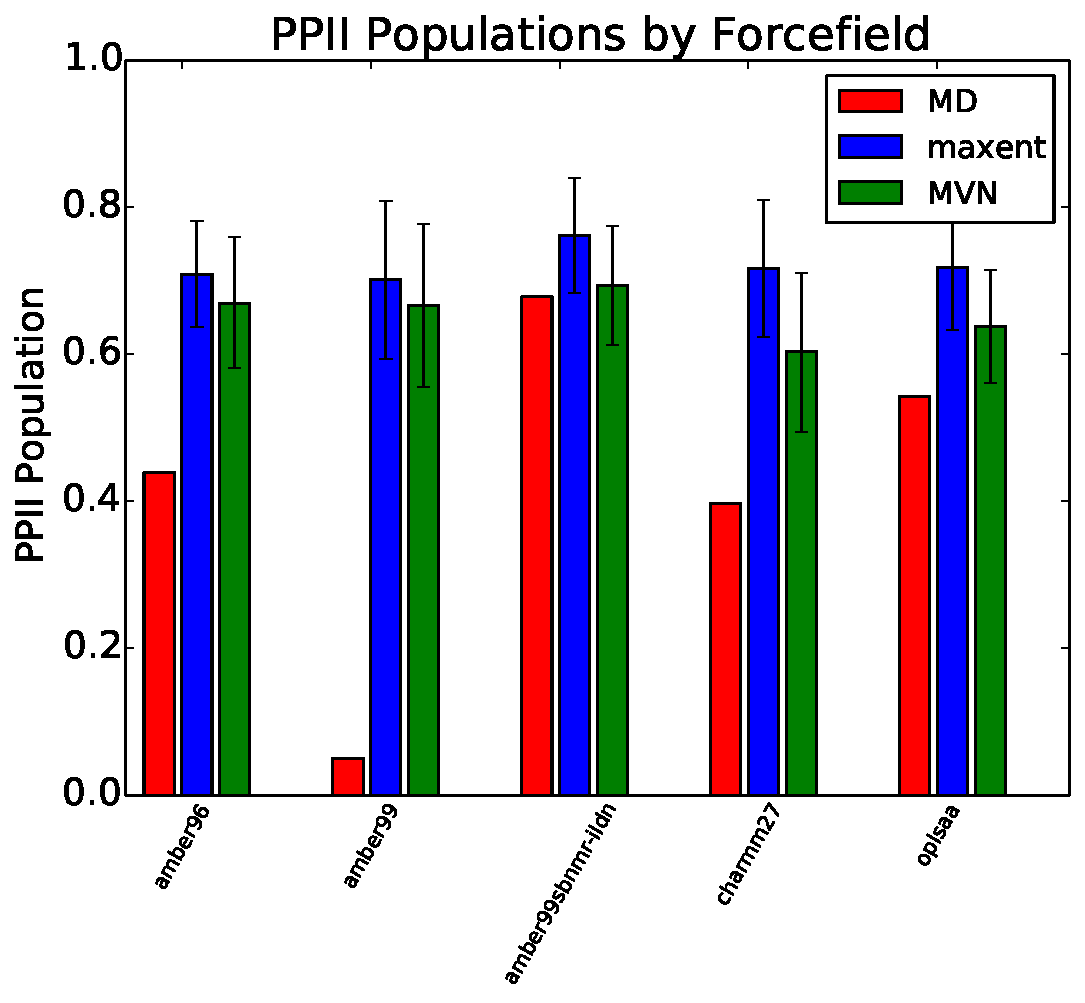
\includegraphics[width=7.5cm]{figures/state_0_by_forcefield_priors.pdf}
}

\subfigure[]{
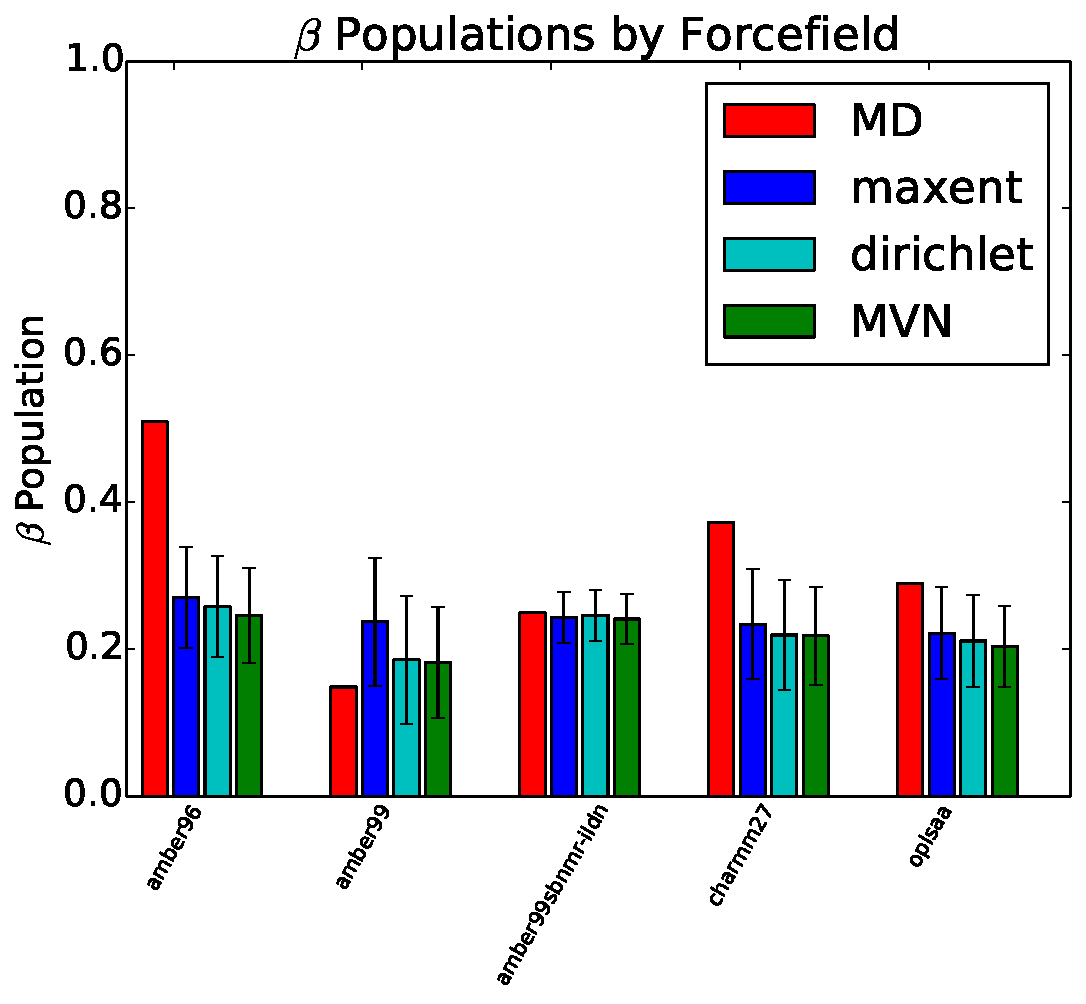
\includegraphics[width=7.5cm]{figures/state_1_by_forcefield_priors.pdf}
}
\subfigure[]{
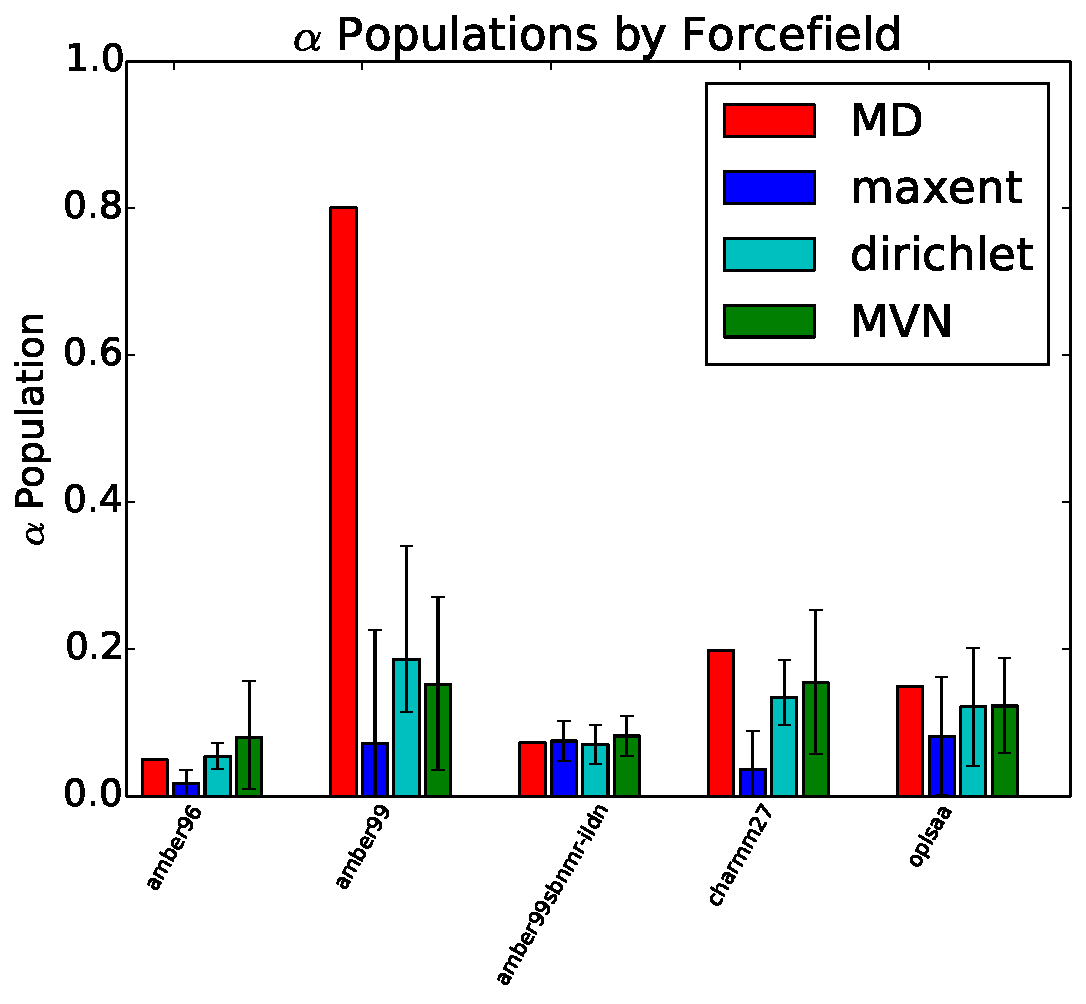
\includegraphics[width=7.5cm]{figures/state_2_by_forcefield_priors.pdf}
}
\caption{
MD and BELT (maxent, Dirichlet, and MVN priors) conformational propensities (for central alanine residue) in each force field.  
}
\label{figure:ALA3}
\end{figure}


\begin{figure}
\subfigure[]{
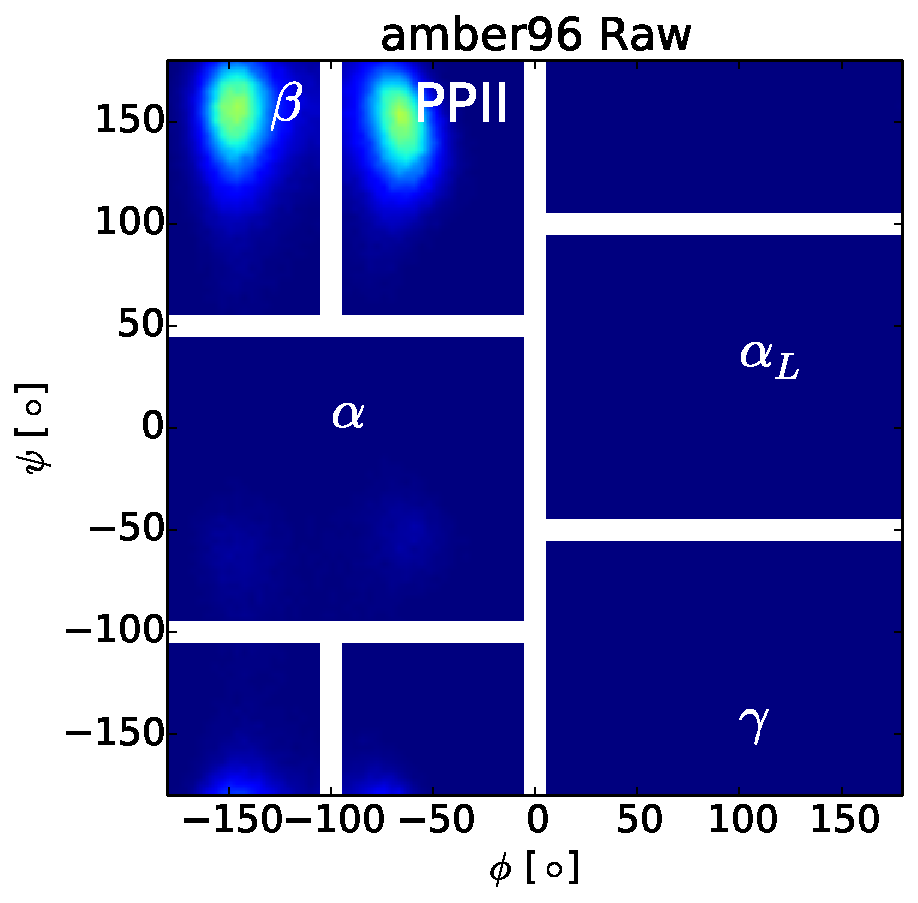
\includegraphics[width=5.05cm]{figures/ALA3_rama_amber96_raw.pdf}
}
\subfigure[]{
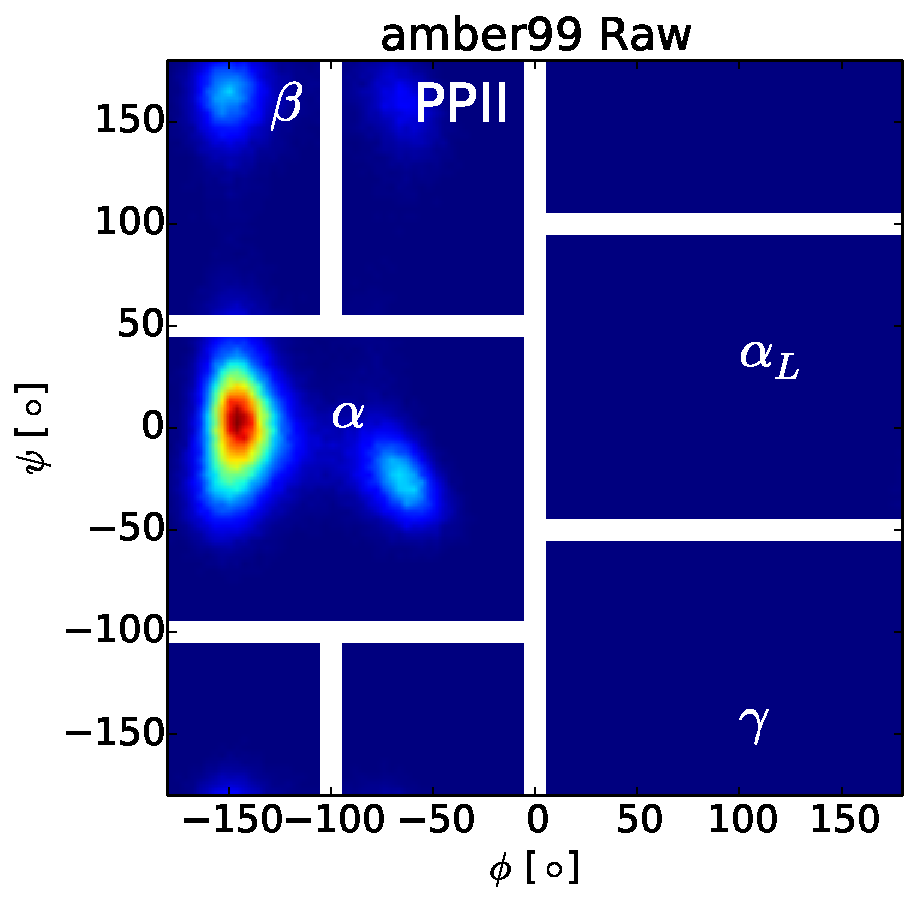
\includegraphics[width=5.05cm]{figures/ALA3_rama_amber99_raw.pdf}
}
\subfigure[]{
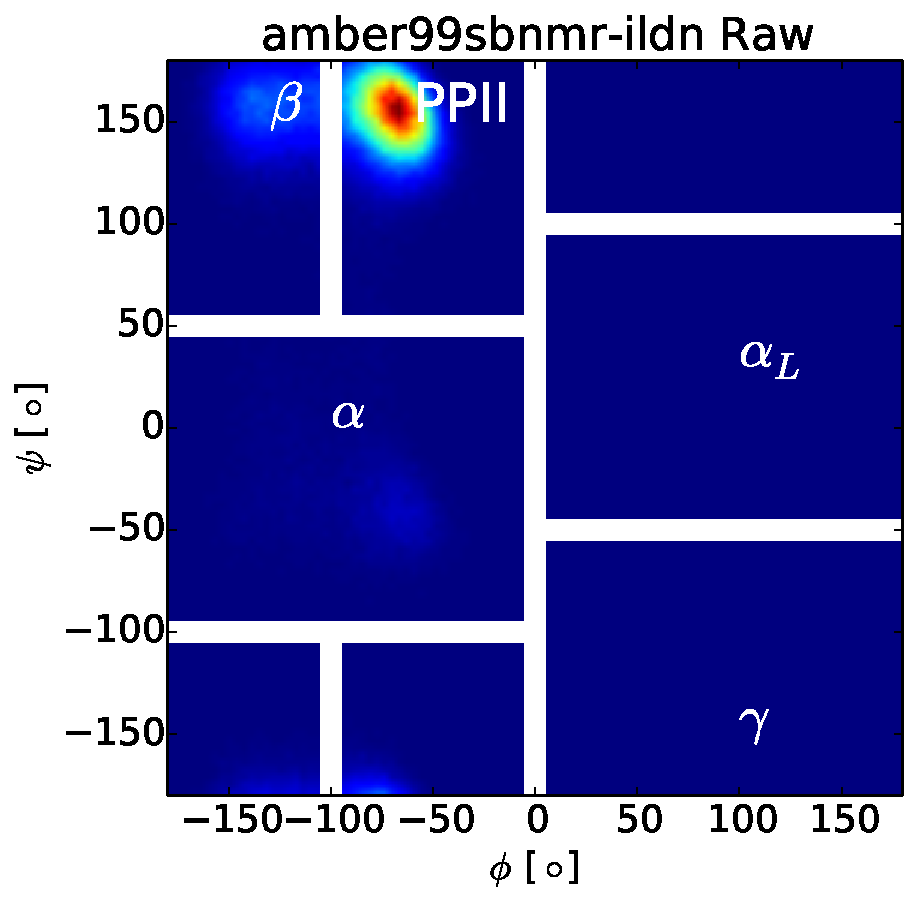
\includegraphics[width=5.05cm]{figures/ALA3_rama_amber99sbnmr-ildn_raw.pdf}
}

\subfigure[]{
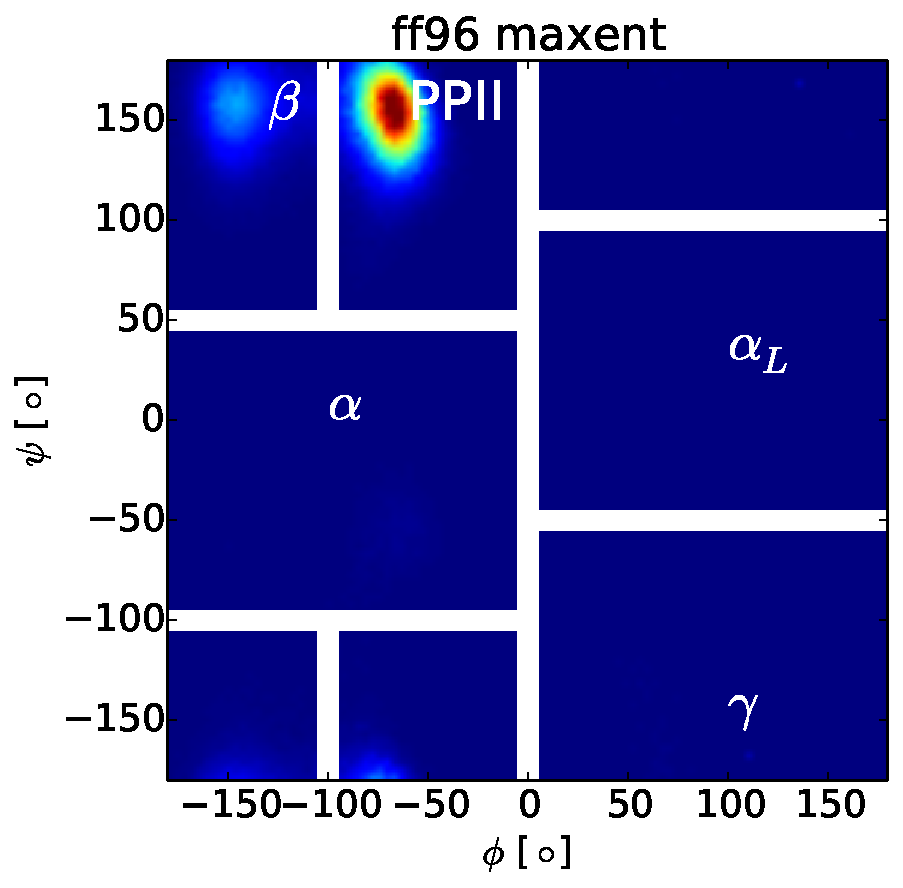
\includegraphics[width=5.05cm]{figures/ALA3_rama_amber96_maxent_belt.pdf}
}
\subfigure[]{
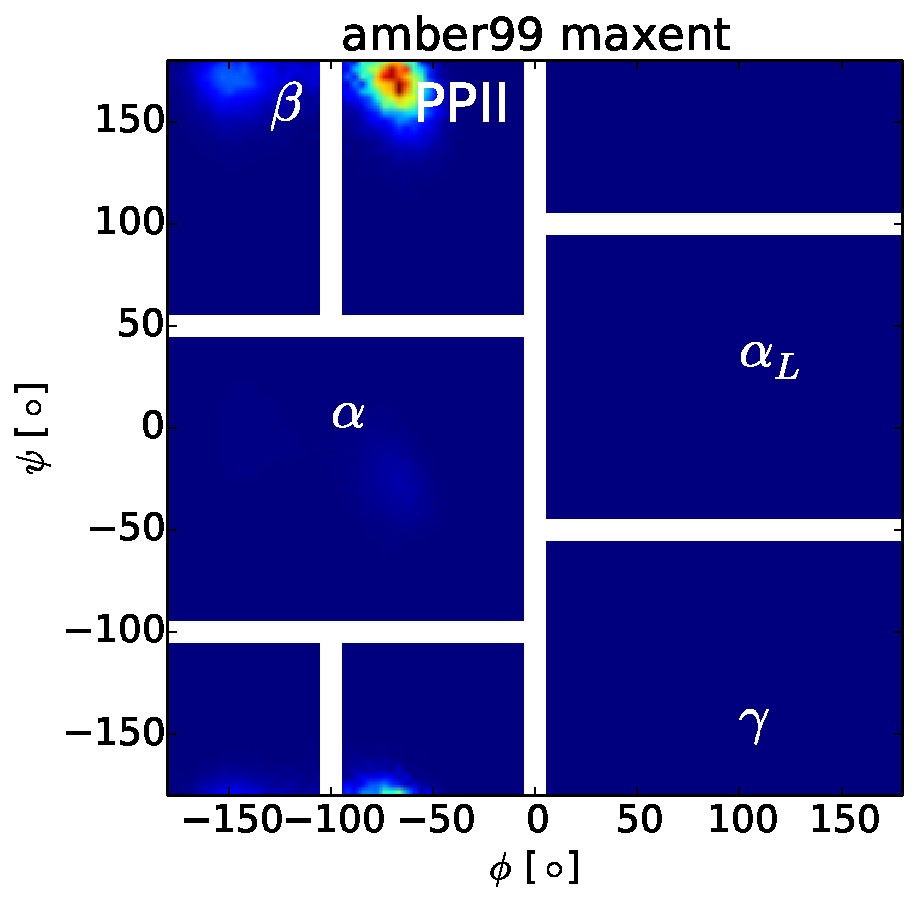
\includegraphics[width=5.05cm]{figures/ALA3_rama_amber99_maxent_belt.pdf}
}
\subfigure[]{
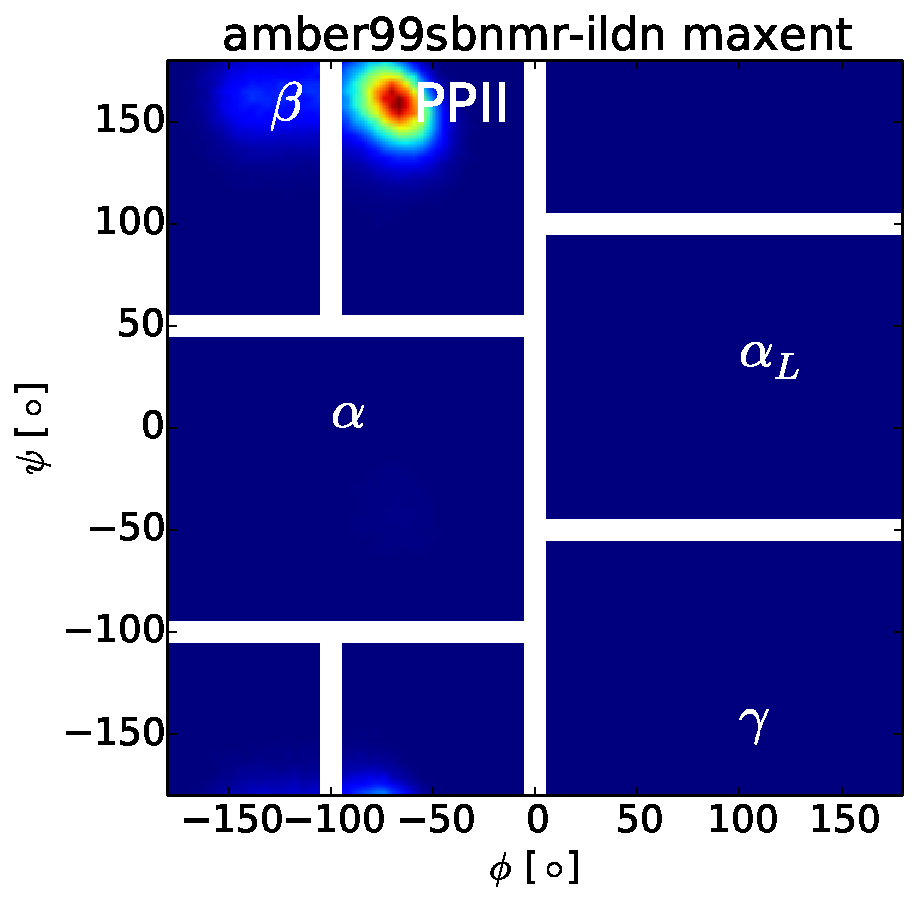
\includegraphics[width=5.05cm]{figures/ALA3_rama_amber99sbnmr-ildn_maxent_belt.pdf}
}

\subfigure[]{
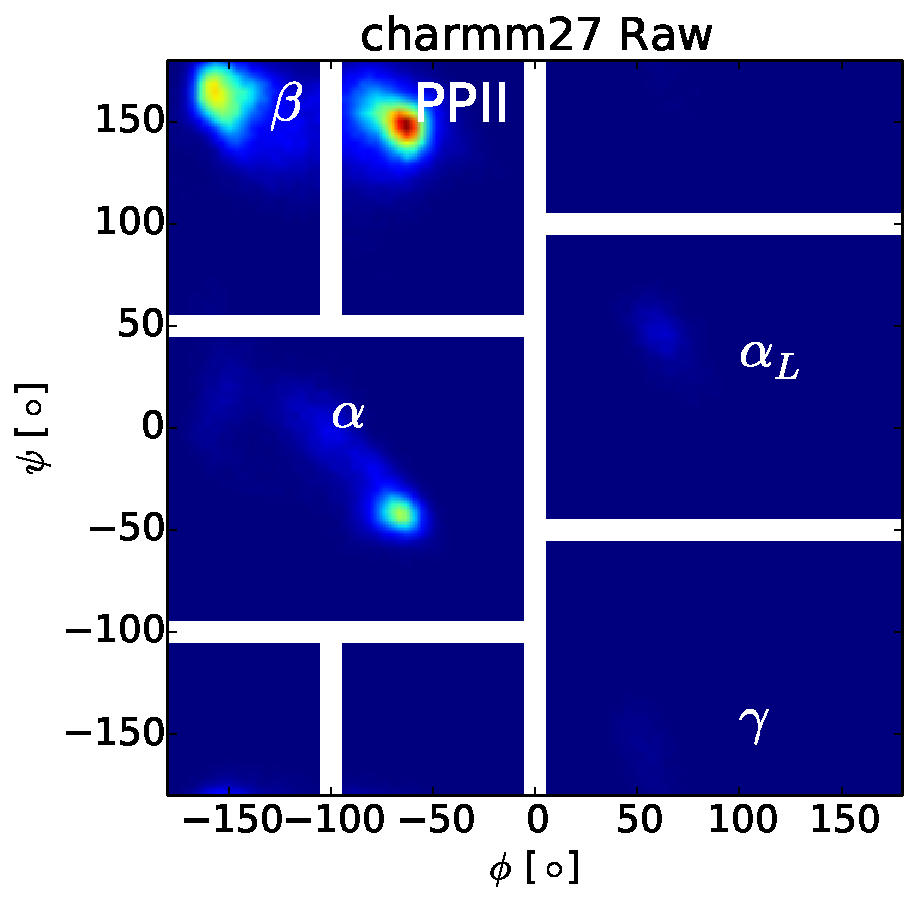
\includegraphics[width=5.05cm]{figures/ALA3_rama_charmm27_raw.pdf}
}
\subfigure[]{
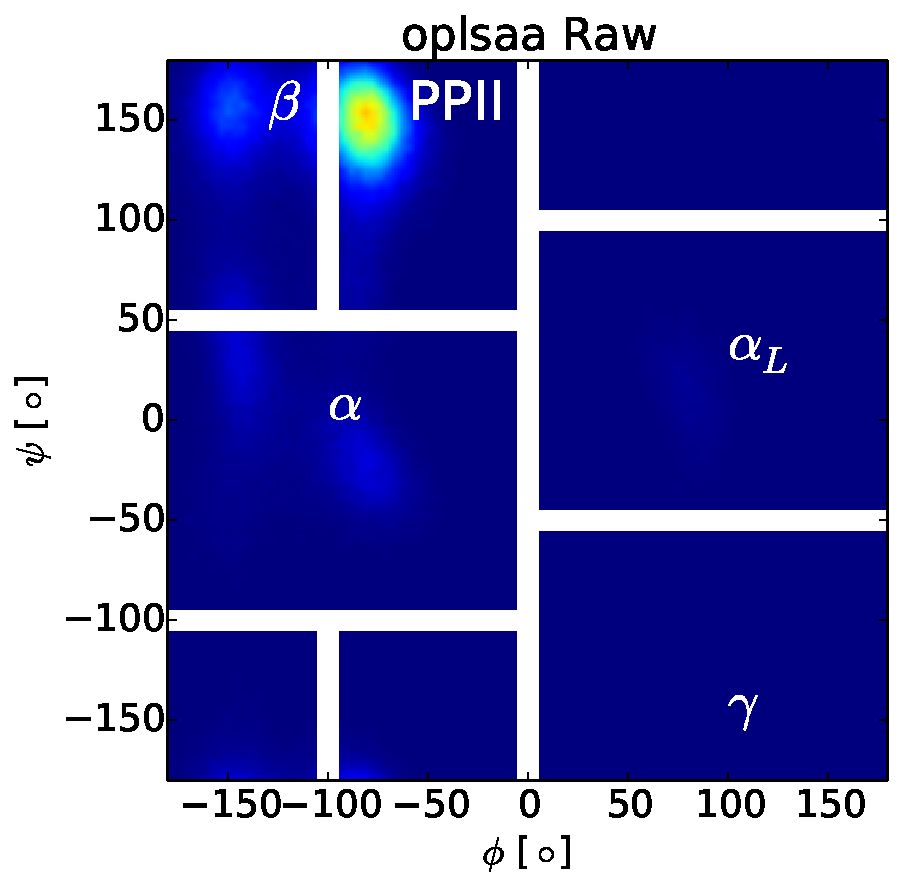
\includegraphics[width=5.05cm]{figures/ALA3_rama_oplsaa_raw.pdf}
}

\subfigure[]{
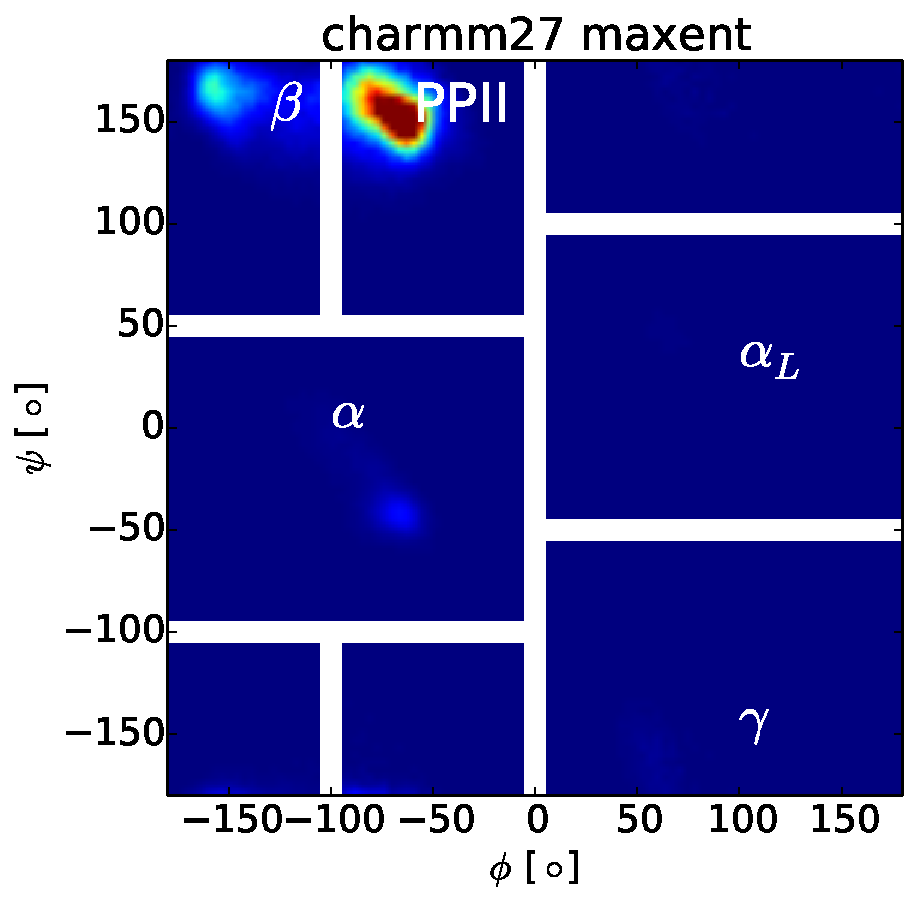
\includegraphics[width=5.05cm]{figures/ALA3_rama_charmm27_maxent_belt.pdf}
}
\subfigure[]{
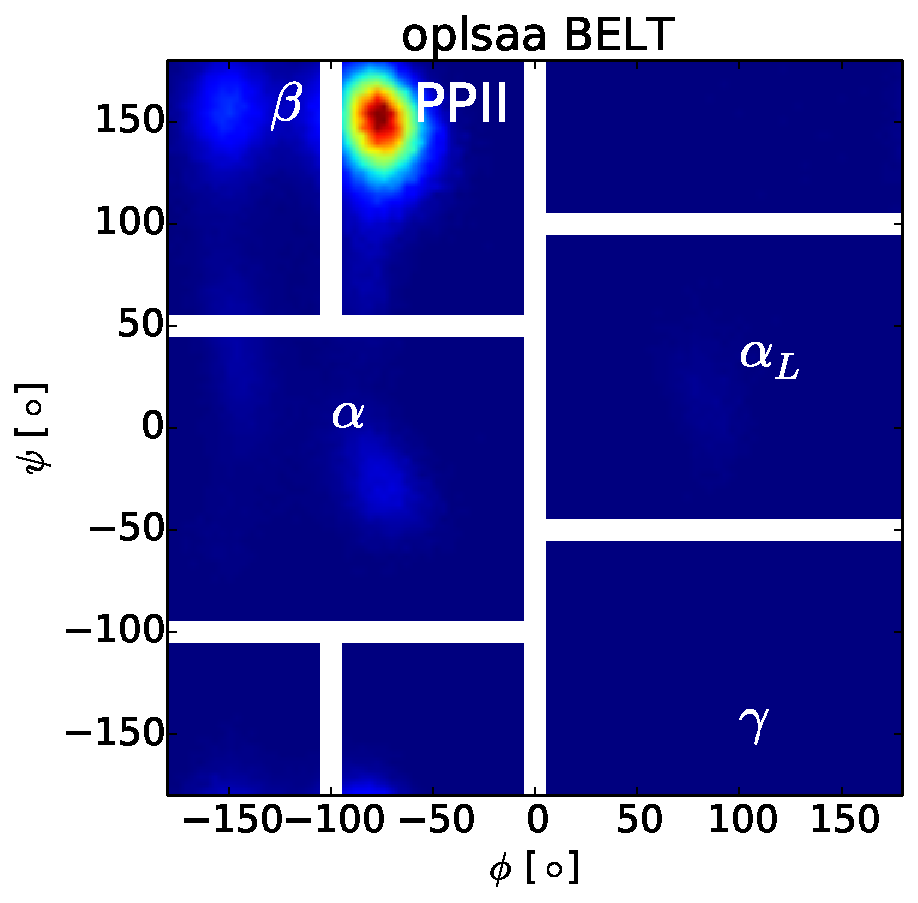
\includegraphics[width=5.05cm]{figures/ALA3_rama_oplsaa_maxent_belt.pdf}
}
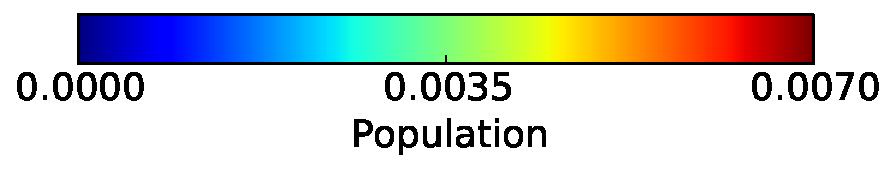
\includegraphics[width=5.05cm]{figures/ALA3_rama_colorbar.pdf}


\caption{
Ramachandran plots of MD and BELT (maxent prior) ensembles for each force field; additional priors are shown in Fig. S1.  The jagged appearance of the amber99 BELT model is due to limited sampling of PPII configurations in that forcefield.  
}
\label{figure:Rama}
\end{figure}

Several independent experimental studies have shown that short alanine peptides prefer the polyproline type helix (PPII) in solution  \citep{Grdadolnik2011, Graf2007, Avbelj2006}.  Most molecular dynamics force fields, however, are known to underpopulate the PPII state  \citep{Graf2007,beauchamp2012protein, nerenberg2011, best2008}.  Our trialanine simulations recapitulate this known deficiency (Fig. \ref{figure:ALA3}; red), with amber96 showing a strong $\beta$ bias (Fig. \ref{figure:ALA3}b) and amber99 showing a strong $\alpha$ bias (Fig. \ref{figure:ALA3}c).  However, combining simulation and experiment leads to conformational ensembles that are robust to differences in force field and prior (Fig. \ref{figure:ALA3}; blue, cyan, and green).  Full Ramachandran plots of the $(\phi, \psi)$ preferences (Fig. \ref{figure:Rama}) reveal similar features in all five BELT models.  

\subsection*{Bayesian Inference allows Ambiguous Experiments}

BELT allows the full characterization of posterior distributions using MCMC.  Most previous approaches, however, have focused on obtaining point estimates of conformational ensembles  \citep{rozycki2011saxs,  Graf2007}.  In many cases, however, ambiguous experimental data preclude a point-estimate of the conformational ensemble.  To illustrate this point, we plot the measured  \citep{Graf2007} value of $^3J(H_NH_\alpha)$ in the context of the Karplus \citep{vogeli2007limits} equation relating $\phi$ to $^3J(H_NH_\alpha)$.  The measured coupling corresponds to four different values of $\phi$ (Fig. \ref{figure:Ambiguity}a), suggesting that a point estimate is inappropriate for modeling conformations or ensembles.  As a concrete example of bimodality, we calculated the posterior distribution of $PP_{II}$ populations for the oplsaa force field reweighted with two NMR measurements (Fig. \ref{figure:Ambiguity}b).  The observed bimodal distribution indicates the need to fully characterize the posterior 
distribution.  

\begin{figure}
\subfigure[]{
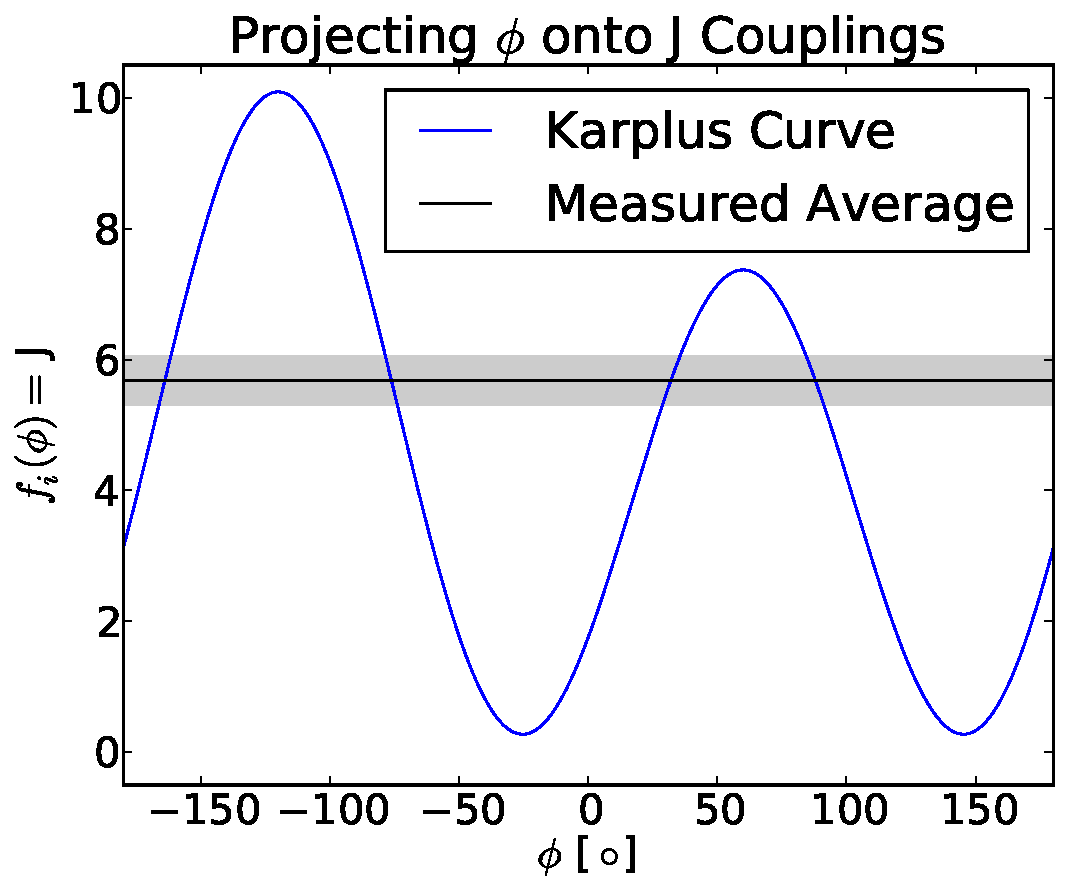
\includegraphics[width=7.5cm]{figures/single_karplus.pdf}
}
\subfigure[]{
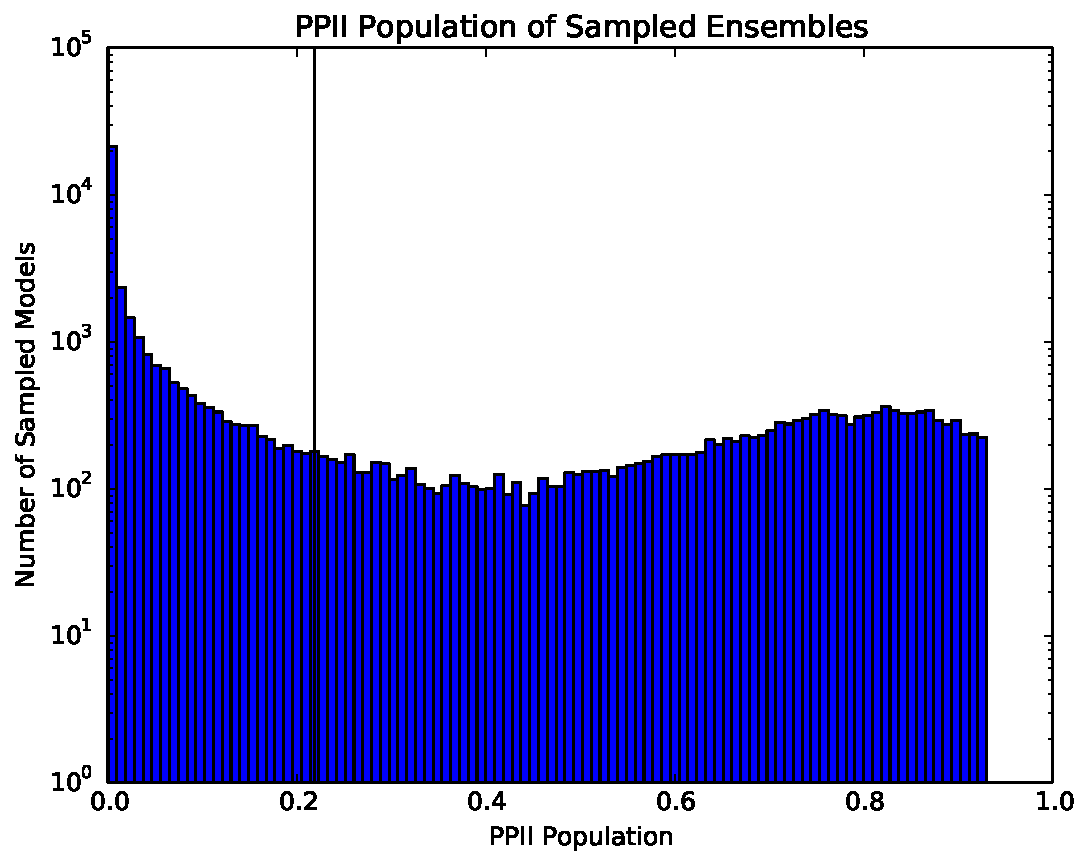
\includegraphics[width=7.5cm]{figures/oplsaa_PPII_histogram.pdf}
}
\caption{
(a).  The Karplus equation connecting the backbone torsion $\phi$ to $^3J(H_NH_\alpha)$ is ambiguous; the observed value of $^3J(H_NH_\alpha)$ is consistent multiple conformations.  (b).  BELT modeling (oplsaa force field) with two measurements ($^3J(H_N C_\beta)$, $C_\beta$ chemical shift) shows a bimodal posterior.  The mean is shown as a black line; due to the bimodality, the mean value lies near a population minimum.
}
\label{figure:Ambiguity}

\end{figure}



\section*{Discussion}

The advantages of the present work are fivefold.  First, we focus on equilibrium experimental measurements, such as chemical shifts and scalar couplings.  Such experiments are straightforward to perform and interpret.  Chemical shifts in particular are the most fundamental NMR observable and are widely available.  Although chemical shift modeling has previously been demonstrated \cite{shen2008consistent} in the context of structure prediction, the current work uses chemical shifts (and scalar couplings) to estimate conformational ensembles.  Second, previous ensemble studies have focused on point estimates of ensembles \cite{rozycki2011saxs, lindorff2005simultaneous, lange2008recognition}, whereas we demonstrate Bayesian inference of conformational ensembles--allowing rigorous estimates of equilibrium and structural properties and their associated uncertainties.  Third, although other Bayesian ensemble inference techniques have been described \cite{fisher2010}, the current work demonstrates a 
new approach to reducing the size of the parameter space.  Fourth, the robustness of BELT models to the initial force field indicates that, for the first time, simulation based models can make robust predictions that are unbiased by forcefield inaccuracy.  Finally, we have implemented our methods in a fully-documented, open-source library (FitEnsemble: \url{https://github.com/kyleabeauchamp/FitEnsemble}), which will be of use to researchers in the field.  

\subsection*{Structural (Ensemble?) Biology}

Why model structural ensembles, rather than just structures?  At least three compelling reasons favor ensembles.  First, biological molecules are multi-state machines that fold, unfold, bind ligands, aggregate, and change conformation.  Biology is controlled by the relative populations of these states.  Ensembles capture aspects of these phenomena by encoding equilibrium populations with structures.  A second argument for ensemble modeling is fidelity to experiment.  Most solution experiments measure ensemble average equilibrium properties--chemical shifts, scalar couplings, NOEs, SAXS, and FRET are reasonably well-described as equilibrium properties.  A truly quantitative connection to these measurements requires modeling the equilibrium ensemble.  Finally, recent advances in atomistic simulation  \citep{hess2008, pronk2013gromacs, eastman2012openmm, eastman2010openmm}, special-purpose hardware  \citep{Shaw2008}, and distributed computing analysis  \citep{emma, msmb2} have enabled atomistic simulations to 
reach the millisecond timescale  \citep{voelz2010, bowman2011atomistic, shaw2010, Shaw2011}; the computational cost of ensemble modeling is quickly becoming manageable.

One might argue that structural ensembles are unnecessary because many proteins occupy a single state under physiological conditions.  For such proteins, it is probably safe to enforce single state behavior, as is done in current modeling approaches. However, we suggest that the number of states be inferred--not assumed.  


\subsection*{Resolving Fine Structure May Require Improved Observables}

The five BELT ensembles show near-quantitative agreement in $\alpha$, $\beta$, and $PP_{II}$ populations (Fig. \ref{figure:ALA3}).  However, the finer details of each Ramachandran plot (Fig. \ref{figure:Rama}) suggest subtle differences between the 
five models.  Because all five BELT ensembles show excellent agreement with experiment (Fig. \ref{figure:ChiSquared}), we conclude that current predictors of chemical shifts and scalar couplings are insufficiently precise to resolve (and falsify) subtle force field differences.  The most obvious such difference is the width, shape, and orientation of the $PP_{II}$ basin.  Most strikingly, amber96 and oplsaa have $PP_{II}$ basins that are vertically oriented, while amber99, amber99sbnmr-ildn, and charmm27 show diagonally oriented $PP_{II}$ basins.  This highlights the need for more sensitive connections between simulation and experiment, such as chemical shift and scalar coupling models.  It is also possible that the NMR measurements contain insufficient information to resolve such level of differences, which would indicate the need for additional measurements.  


\subsection*{Comparison to Previous Ensemble Methods}

Most previous ensemble modeling efforts involve a protocol with three key ingredients: state decomposition, a $\chi^2$ objective function, and population inference on the clusters.  For example, this general recipe describes the approach used in previous analyses of homopeptides  \citep{Graf2007}, the EROS technique for SAXS modeling  \citep{rozycki2011saxs}, and the Bayesian Weighting (BW) formalism  \citep{fisher2010}.  Note that of these three techniques, BW fully characterizes the posterior distribution via MCMC; below we therefore focus our attention on BW as it is most directly comparable to BELT in scope and purpose.

The primary disadvantage of previous techniques is the need for a state decomposition, which can be defined either by hand or by clustering.  Working with a given state decomposition can introduce two different errors, depending on the number  and quality of states.  In the limit of few states, clustering can overly coarsen the system of interest, possible preventing the model from reproducing multiple experimental observables.  At the other extreme, too many states leads to a large number of parameters to be estimated. This will lead to poor generalization performance and large errors when predicting experiments not used to train the model, as well as reliance on a subjective choice of how many states is appropriate.  One symptom of this regime is discontinuity in conformational populations. For example, imagine two nearby conformations at the boundary between two BW states--one conformation on each side of the boundary.  In BW, the populations of each conformation could fluctuate dramatically with the corresponding 
state populations.  In BELT, however, the two conformations will have nearly identical populations if the predicted observables vary smoothly.

BELT avoids arbitrary state decompositions by projecting simulations onto a basis defined by the predicted experimental observables.  The advantage of working in this basis are threefold. First, in BELT, one estimates a single parameter ($\alpha_i$) for each experimental observable.  If the number of experiments is small, as is often the case, the inference problem involves only a few parameters.  Second, the predicted observables are a natural basis for biophysical calculations, in that the predicted observables are the fundamental connection between simulation and experiment.  Working in this basis allows direct connection to experiment and often provides insight into the molecular interactions driving biophysical phenomena.  For example, the projection onto observables could be used to rationally infer force field parameters--essentially a Bayesian version of the ForceBalance method  \citep{wang2012, wang2013systematic}.  Third, in the limit of exact measurements, BELT reduces to a previous  \citep{chodera2012} maximum entropy approach (see Appx. S1).  

We also point out some surprising differences between BELT and BW-like methods.  BW-like methods have the interesting property that the in-state means of features are preserved.  More precisely, suppose that $\chi_s(x)$ is the indicator function of a conformational state $s$.  Then in-state averages of the form $<\chi_s(x)>^{-1} <h(x) \chi_s(x)>$ do not depend on the reweighted populations.  BELT, however, does not preserve the in-state averages; in fact, this property is the direct result of BELT's connection to maximum entropy modeling (see Appx. S1 and ref.  \citep{chodera2012}).  The effect of this property is that the peaks of reweighted histograms are slightly shifted relative to the raw MD results, as observed in Fig. \ref{figure:Hist}.   

\section*{Limitations of BELT}

There are several limitations of the BELT method.  Most obvious is that BELT can only reweight existing simulations.  The force field used must be sufficiently accurate to sample experimentally-consistent conformations.  For example, the trialanine simulations in ff99 sampled PPII conformations--the experimentally dominant state--only about five percent of the time.  Achieving accurate predictions using poor force fields may require orders of magnitude more MD sampling.  The same increased sampling requirements apply as one attempts to fit many measurements simultaneously.  In the worst-case scenario, fitting $n$ measurements could require MD datasets whose size grows exponentially with $n$.  A second limitation in BELT is its computational cost.  In the present calculations, MCMC sampling for each model took approximately 24 hours.  These datasets used included six measurements and approximately 250,000 conformations.  Because using additional conformations is computationally prohibitive, BELT ensembles are essentially limited to resolving states that have populations of $250000^{-1}$--a free energy difference of approximately $7 kcal mol^{-1}$.  A third limitation is the independent normal approximation used in BELT's error model (see Appx. S3).  Most sophisticated frameworks may be possible, including the Bayesian formalisms from the Nilges group \citep{rieping2005, habeck2006, habeck2005bayesian}.  


The BELT method can be extended in several ways.  We have already worked out some of these extensions.  In Appx. S3, we derive an approximate correction for working with dependent data.  Another obvious extension is the use of non-normal error models.  These models can be directly inserted into the current framework by replacing the $\chi^2$ term in the likelihood with some other loss function.  More sophisticated models could separately treat the uncertainties associated with predicting observables and the uncertainties of conformations.  This would replace the regularization and Bayesian Bootstrapping (Appx. S6) approaches used herein.  Another promising avenue is to combine Bayesian modeling of structural ensembles with Bayesian models for experimental observables.  A Bayesian formalism for NMR experiments has previously been developed  \citep{rieping2005, habeck2006, habeck2005bayesian}; connecting BELT to these methods may be straightforward.  


\section*{Conclusion}

Bayesian Energy Landscape Tilting allows the simultaneous characterization of structural and equilibrium properties.  Through its use of MCMC, BELT is robust to ambiguous experiments and provides rigorous uncertainty estimates, as illustrated here in the case of a simple tripeptide system.  BELT models constructed with a handful of NMR measurements correct significant force field bias and provide generalizable, force field independent trialanine ensembles.  The principled combination of simulation and experiment will enable robust, incisive predictions of the atomic-scale behavior of macromolecules.  


\section*{Acknowledgements}

We thank John Chodera, TJ Lane, Frank Cochran, Pehr Harbury, Xuesong Shi, and Dan Herschlag for helpful discussions.  

\bibliography{belt}


\end{document}